

\tikzset{every picture/.style={line width=0.75pt}} %set default line width to 0.75pt        

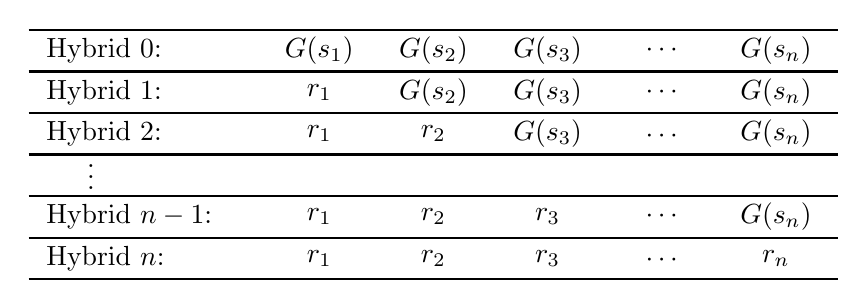
\begin{tikzpicture}[x=0.75pt,y=0.75pt,yscale=-1,xscale=1]
%uncomment if require: \path (0,300); %set diagram left start at 0, and has height of 300

%Straight Lines [id:da6691560220286636] 
\draw    (0,0) -- (390,0) ;
%Straight Lines [id:da14937141719479574] 
\draw    (0,20) -- (390,20) ;
%Straight Lines [id:da19416400836028047] 
\draw    (0,40) -- (390,40) ;
%Straight Lines [id:da4673631663401927] 
\draw    (0,60) -- (390,60) ;
%Straight Lines [id:da20994958717605572] 
\draw    (0,80) -- (390,80) ;
%Straight Lines [id:da07444150912485936] 
\draw    (0,100) -- (390,100) ;
%Straight Lines [id:da5538446859570711] 
\draw    (0,120) -- (390,120) ;

% Text Node
\draw (7,10) node [anchor=west] [inner sep=0.75pt]   [align=left] {Hybrid $\displaystyle 0$:};
% Text Node
\draw (7,30) node [anchor=west] [inner sep=0.75pt]   [align=left] {Hybrid $\displaystyle 1$:};
% Text Node
\draw (7,50) node [anchor=west] [inner sep=0.75pt]   [align=left] {Hybrid $\displaystyle 2$:};
% Text Node
\draw (7,90) node [anchor=west] [inner sep=0.75pt]   [align=left] {Hybrid $\displaystyle n-1$:};
% Text Node
\draw (7,110) node [anchor=west] [inner sep=0.75pt]   [align=left] {Hybrid $\displaystyle n$:};
% Text Node
\draw (140,10) node    {$G( s_{1})$};
% Text Node
\draw (195,10) node    {$G( s_{2})$};
% Text Node
\draw (250,10) node    {$G( s_{3})$};
% Text Node
\draw (305,10) node    {$\cdots $};
% Text Node
\draw (360,10) node    {$G( s_{n})$};
% Text Node
\draw (140,30) node    {$r_{1}$};
% Text Node
\draw (140,50) node    {$r_{1}$};
% Text Node
\draw (140,90) node    {$r_{1}$};
% Text Node
\draw (140,110) node    {$r_{1}$};
% Text Node
\draw (195,30) node    {$G( s_{2})$};
% Text Node
\draw (250,30) node    {$G( s_{3})$};
% Text Node
\draw (250,50) node    {$G( s_{3})$};
% Text Node
\draw (305,30) node    {$\cdots $};
% Text Node
\draw (305,51.2) node    {$\cdots $};
% Text Node
\draw (305,90) node    {$\cdots $};
% Text Node
\draw (305,111.2) node    {$\cdots $};
% Text Node
\draw (360,30) node    {$G( s_{n})$};
% Text Node
\draw (360,50) node    {$G( s_{n})$};
% Text Node
\draw (360,90) node    {$G( s_{n})$};
% Text Node
\draw (195,50) node    {$r_{2}$};
% Text Node
\draw (195,90) node    {$r_{2}$};
% Text Node
\draw (195,110) node    {$r_{2}$};
% Text Node
\draw (250,90) node    {$r_{3}$};
% Text Node
\draw (250,110) node    {$r_{3}$};
% Text Node
\draw (360,110) node    {$r_{n}$};
% Text Node
\draw (30,67) node    {$\vdots $};


\end{tikzpicture}